\documentclass[twoside]{article}
\usepackage{fleqn,espcrc2}

\usepackage{graphicx}
\usepackage[figuresright]{rotating}

\newcommand\ttbs{\char'134}
\newcommand\AmS{{\protect\the\textfont2
 A\kern-.1667em\lower.5ex\hbox{M}\kern-.125emS}}

\hyphenation{author another created financial paper re-commend-ed  Post-Script}

\title{The physics of the stripe quantum critical point in  the superconducting cuprates}

\author{C. Di Castro, L. Benfatto, S. Caprara,  C. Castellani, and M. Grilli\address{INFM and Dipartimento di Fisica Universit\`{a} di Roma ``La Sapienza'' \\   00185 Rome, Italy}}

\begin{document}

\begin{abstract}

We elaborate on several observable consequences of the Quantum-Critical-Point
scenario. In particular we show that
the strong k-dependent scattering of the quasiparticles with the
quasi-critical charge and spin fluctuations reproduces the main features of
the low-energy spectral weights and of the observed Fermi surfaces. In the
underdoped cuprates the attractive k-dependent charge scattering drives the
formation of the pseudogap at the M points below the crossover temperature
$T^*$. In this context we discuss models for pseudogap formation with
relevant scattering in the particle-particle and particle-hole channels. The
experimental consequences for the pair-fluctuation and for the
pseudogap behavior are investigated.
\vspace{1pc}
\end{abstract}

\maketitle

\section{THE STRIPE QUANTUM CRITICAL POINT SCENARIO}

The non-Fermi-liquid behavior of the normal-state of the cuprates has two
major features depending on the doping $(\delta)$ regimes. Specifically,
(i) near optimal doping no energy scales seem to be present besides the
temperature (e.g. the in-plane resistivity stays linear in $T$ from just
above the critical temperature $T_c$), while (ii) in the underdoped regime,
new energy
scales appear in the form of pseudogaps, which persist well above $T_c$ up to
a doping-dependent crossover temperature $T^*$ \cite{timusk}. Starting in the
deeply underdoped phase, $T_c$ increases with increasing doping and $T^*$
decreases from high values of several hundreds of kelvins until it merges
with $T_c$ near optimal doping. On the other hand, a Fermi-liquid-like
behavior is observed in the overdoped materials. Correspondingly,
many different physical quantities display qualitatively different
behaviors in going from the under- to the optimally and to the over-doped
regimes. As schematically described in Fig. 1, the subdivision of the phase
diagram in three regions naturally arises from the occurrence of an
instability line starting at high temperature in the deeply underdoped phase
and ending at zero temperature in a quantum critical point (QCP) located near
optimal doping.
In this scheme the optimally doped and overdoped regimes would be related to
the quantum critical (QC) and to the quantum disordered (QD) region of the
QCP respectively. The two regions are separated by a crossover line
$\tilde{T}(\delta)$. The underdoped regime corresponds to the (quasi)-ordered
region below the instability line. However, precursor effects of the ordering
could extend up to a higher temperature $T_0(\delta)$.

\begin{figure}
\begin{center}
\includegraphics[width=12pc,height=15pc,angle=-90]{Fig1.ps}
\caption{Schematic structure of the temperature vs. doping $\delta$ phase  diagram around the Stripe-QCP.}
\label{fsmodel}
\end{center}
\end{figure}

It was shown that in strongly correlated systems (e.g., in the
large-U Hubbard model with an
electron-phonon interaction and long-range Coulomb forces) an incommensurate
charge-density-wave instability occurs when the doping is reduced below a
critical value $\delta_c$ \cite{prl95,prb96,jpcs98}. This tendency to order
the charge arises as a compromise between the local tendency towards phase
separation and the electrostatic cost to segregate charged carriers \cite{PS}.
For reasonable values of the parameters this
instability line starts near optimal doping at zero temperature. In the
underdoped regime this charge ordering tendency occurs below a
doping-dependent $T_{CDW}(\delta)$ instability line. The charge ordering
strongly mixes with spin degrees of freedom and gives rise to the so-called
stripe phase.

As shown in Ref. \cite{prl95,jpcs98} a crucial consequence of the stripe
formation
is the occurrence nearby the instability of a singular effective interaction,
strongly dependent on momentum, doping, and temperature:
\begin{equation}
\Gamma ({\bf q},\omega) \approx
\tilde{U} - \frac{V}{\kappa^{2}+ \vert{\bf q} - {\bf q}_c \vert^2 - i\gamma \omega}
\label{fitgamlr}
\end{equation}
where $\tilde{U}$ is the residual repulsive interaction between the
quasiparticles, $\gamma$ is a damping parameter, and ${\bf q}_c$ is the
wavevector of the CDW instability. The crucial parameter
$\kappa^2=\xi_c^{-2}$ is
the inverse square of the correlation length of charge
order and provides a measure of the distance from criticality.
At $T=0$, in the overdoped regime, $\kappa^2$ is linear in the
doping deviation from the critical concentration, $\kappa^2=a(\delta-
\delta_c)$. In Ref. \cite{prl95} the instability was found at
$\delta_c\approx 0.2$, with $q_c \sim 1$. On the other hand, in the QC region
above $\delta_c$, $\kappa^2\sim T$, according to the behavior of a Gaussian
QCP. In the underdoped regime $\kappa^2$ vanishes approaching the
instability line $T_{CDW}(\delta)$.

The occurrence of singular interactions near the QCP and near the
instability line determines the physical properties of the
cuprates. In particular, the non-Fermi-liquid behavior characteristic of the
optimally doped materials is a signature of the QCP \cite{prl95}. In the next
section we report on some spectroscopic
consequences of the strong scattering mediated by charge fluctuations near
optimal doping. On the other hand in the overdoped region the term
$\kappa^2=a(\delta-\delta_c)$ reduces the scattering and determines a region
of Fermi-liquid behavior. In the underdoped compounds, when the instability
line $T_{CDW}$ is approached, a singular scattering between the quasiparticles
is again mediated by the charge fluctuations at wavevectors
${\mbox{\bf $q$}} \approx{\mbox{\bf $q$}}_c$. Thus the region near
$T_{CDW}(\delta)$ is characterized by a strong effective interaction both in
the particle-particle (p-p) and the particle-hole (p-h) channels, with a new
doping-dependent energy scale. In both cases a pseudogap is an expected
outcome, as it will be discussed in Section 3.

\section{SPECTRAL PROPERTIES NEAR OPTIMAL DOPING}

The charge fluctuations couple with spin degrees of freedom since in the
hole-poor regions the system is locally closer to half-filling where
antiferromagnetic correlations are more pronounced. Both charge and spin
fluctuations then mediate a nearly singular scattering between the
quasiparticles, strongly affecting the spectral properties. In order to
compare the outcomes of this scattering with the ARPES experiments, mostly
performed on optimally doped Bi2212 \cite{SAINI}, we assumed \cite{CAPRARA} a
tight-binding model with the band parameters commonly accepted for this
material.
The exchange of QC charge fluctuations at wavevectors ${\bf q}_c=\pm
(0.4\pi,-0.4\pi)$, and QC antiferromagnetic spin fluctuations at ${\bf q}_s=
(\pi,\pi)$ was then considered within a perturbative approach. Since in
general the critical wavevector is model
and doping dependent, the present choice of ${\bf q}_c$ was suggested
to match the experiments \cite{SAINI}.
The resulting single-particle spectra are
characterized by (i) a transfer of spectral weight from the quasiparticle
peak to the incoherent shadow peaks; (ii) a redistribution of the
low-energy spectral weight with a modification of the FS; (iii) a strong
anisotropic suppression of spectral weight around the M points
$(\pm\pi,0)$ and $(0,\pm\pi)$. All these
features have a counterpart in the experiments.

In this framework one can also investigate the bilayer structure of Bi2212
and explain the puzzling absence of bonding-antibonding band
splitting. According to the band calculations \cite{andersen},
we introduced \cite{CAPRARA2} a k-dependent interplane hopping
$t_\perp({\bf k})=t_\perp |\gamma_{\bf k}|$
with $\gamma_{\bf k}={1\over 2}(\cos k_x -\cos k_y )$.
$t_\perp({\bf k})$ is large near the M points only. The intraplane scattering,
however, mostly reduces the quasiparticle spectral weight near the M points.
Thus, within our scenario, the absence of detectable band splitting in ARPES
spectra follows directly from the in-plane spectral properties.

The interaction mediated by the quasicritical fluctuations also provides an
effective pairing mechanism. In this
regard approaching the superconducting region from the overdoped regime, the
doping and the temperature dependences of the $\kappa^2$ term in the QD and QC
regimes give rise to a non-trivial increase of $T_c$ followed by a
saturation around optimal doping \cite{prb96}. The more involved case of the
underdoped regime, with pseudogap formation will be discussed in the next
section.

\section{PARTICLE-PARTICLE AND PAR\-TI\-CLE-HOLE PSEUDOGAP}

The effect of the stripe instability can be more dramatic in underdoped
materials, when the system approaches the instability line at temperatures
$T\sim T_{CDW}(\delta)$. In this case, near $T_{CDW}(\delta)$ the critical
fluctuations at
wavevectors near ${\bf q}_c$ can mediate a large effective interaction
between the quasiparticles states ${\bf k}$ and ${\bf k'}$
such that ${\bf k}-{\bf k'}\sim{\bf q}_c$. The generic outcome is that
states of the Fermi surface near the M points are strongly interacting, while
quasiparticles around the diagonals ($\Gamma-X$ and $\Gamma-Y$ directions)
are less affected. This finds a correspondence in ARPES experiments
\cite{marshall,ding}, where at $T^*$ the Leading Edge shift ($LE$) starts to
develop near the M points. Indeed the strong interaction near the M points
can give rise to pairing and gaps both in the p-p and p-h channels. Although
it is quite natural that both channels contribute to the formation of the
pseudogap below
the crossover temperature $T^*$, the two limiting cases, when a single
channel (either p-p or p-h) dominates the pseudogap formation, are simpler to
analyze and each one of them shows relevant aspects of the physics of the
cuprates.

In the first mechanism we propose, the pseudogap opens due to incoherent
pairing in the p-p channel. The strong momentum dependence of the effective
interaction (\ref{fitgamlr}) plays in this regard a crucial role in selecting
the quasiparticle states which are most strongly paired. This leads to
non-trivial fluctuation effects, because strongly paired states near the M
points coexist with weakly interacting quasiparticles along the diagonals.
This situation is quite different from the case described by a single
superconducting order parameter $\Delta ({\bf k})=\Delta_s g({\bf k})$. In
the present case, indeed, the momentum dependence of the effective pairing
interaction not only produces the k structure of $g({\bf k})$, but also
confers different fluctuation properties {\em in k-space} to the Cooper
pairs depending on their strongly or weakly paired character. This physical
situation has recently been described within a two-gap model \cite{twogap}.
In this latter framework, incoherent tightly bound Cooper pairs around the M
points are formed at $T^*$, while phase coherence is established at a lower
temperature $T_c$ by coupling to the stiffness of the weakly bound pairs near
the diagonal directions.

\begin{figure}
\begin{center}
\includegraphics[width=12pc,height=15pc,angle=-90]{Figtc.ps}
\caption{Doping dependence of $T^*$, $T_c$, and the zero-temperature $LE$. We assumed the $T^*(\delta)$ dependence measured in Bi2212 \cite{ding} and used $c=2.5$ and $V=90$ meV to reproduce the experimentally observed values of the $LE$ in the underdoped region and the maximum $T_c$.}
\label{tctstar}
\end{center}
\end{figure}

The scattering in the p-h channel can provide an additional mechanism for the
pseudogap formation. If this happens, the issue arises of the interplay
between the preformed p-h pseudogap and an additional BCS pairing for the
weakly interacting quasiparticles. While this issue was discussed in Ref.
\cite{nozieres} for a simple isotropic pseudogap, in Ref. \cite{benfatto} a
specific band structure is considered, which includes a preformed k-dependent
gap. The whole complication of the strong scattering around the M points is
schematized by this preformed p-h gap $\Delta_0(\delta,T) \gamma_{\bf k}$,
which separates the conduction and the valence band, and vanishes at the
points $(\pm \pi/2,\pm \pi/2)$. Each band has a width $4t\simeq 1$ eV, $t$
being the nearest-neighbor hopping. We assume $T^*(\delta)$ as the critical
line for the preformed gap formation and take $\Delta_0(\delta,T)=c
T^*(\delta) g(T/T^*(\delta))$, where $c$ is a fitting parameter, $g(0)=1$,
$g(1)=0$, and $g(x)$ interpolates smoothly between these two limits. A
suitable weak pairing $V$ in the Cooper channel promotes a d-wave
superconducting gap $\Delta_s(\delta,T) \gamma_{\bf k}$ in the low valence
band of the hole doped system. The mean-field BCS critical temperature $T_c$
vanishes at $\delta=0$, increases with increasing doping, and reaches a maximum
at $\delta_c$ when the chemical potential crosses the peak which individuates
the pseudogap region in the density of states, and then decreases. Therefore
$T^*$ and $T_c$ merge near optimum doping and the $T_c(\delta)$ curve has the
characteristic bell-shaped form in reasonable agreement with the experiments
(see Fig. 2).

The quasiparticle spectra are characterized by a $LE$, i.e. a finite minimum
distance of the quasiparticle peak from the Fermi level, which persists in
the normal state and is largest at the M points, where $LE\simeq \Delta_0-
|\mu|$. In underdoped SC regime, the $LE$ is controlled by two parameters, as
seen in experiments \cite{PX,TWO}. The M points are dominated by the
normal-state pseudogap, whereas the nodal region are controlled by
$\Delta_s$, which scales as $T_c$. In the overdoped regime the $LE\simeq
\Delta_s$.

The above preformed gap accounts for most of the non-mean-field effects by
the input of a normal-state pseudogap $\Delta_0(\delta,T)$. In particular,
the model yields a phase diagram in good qualitative agreement with the
experiments.

On the other hand, the bifurcation between $T^*$ and $T_c$ nearby optimum
doping is also an outcome of the two-gap model \cite{twogap}. Clearly, the
two models assign a different relevance to the effect of the strong QCP
effective interaction in the p-p and p-h channels, and select just one of the
two channels as the most affected one. It is quite plausible that the stripe
fluctuations will indeed produce non-Fermi-liquid- and non-mean-field-like
effects in both channels. However, whether the results discussed above within
each of the two models should cooperate to produce a better quantitative
description of the cuprates, is still an open problem under investigation.

\begin{thebibliography}{9}

\bibitem{timusk} For a recent review see, {\it e.g.} T. Timusk and 
B. Statt, Rep. Prog. Phys. {\bf 62}, (1999) 61.
\bibitem{prl95} C. Castellani, C. Di Castro, and M. Grilli, 
Phys. Rev. Lett. {\bf 75}, (1995) 4650.
\bibitem{prb96} A. Perali, {\sl et al.}, 
Phys. Rev. B {\bf 54}, (1996) 16216.
\bibitem{jpcs98} C. Castellani, C. Di Castro, and M. Grilli, 
J. Phys. Chem. Solids {\bf 59}, (1998) 1694.
\bibitem{PS} U. L\"{o}w, {\sl et al.}, Phys. Rev. Lett. {\bf 72}, (1994) 1918.
\bibitem{SAINI} N. L. Saini, {\sl et al.}, Phys. Rev. Lett. {\bf 79}, (1997) 
3467.
\bibitem{CAPRARA} S. Caprara, {\sl et al.}, 
Phys. Rev. B {\bf 59}, (1999) 14980.
\bibitem{andersen} O. K. Andersen, {\em et al.}, Phys. Rev. B{\bf 49}, 
(1994) 4145.
\bibitem{CAPRARA2} S. Caprara and M. Grilli, 
Journal de Physique IV (Colloques) {\bf 10}, (1999) 337.
\bibitem{marshall} D. S. Marshall, {\em et al.}, Phys. Rev. Lett. {\bf 76}, 
(1996) 4871.
\bibitem{ding} H. Ding, {\em et al.}, Nature {\bf 382}, (1996) 51; 
J. Phys. Chem. Solids {\bf 59}, (1998) 1888.
\bibitem{twogap} A. Perali, {\sl et al.}, cond-mat/9912363, 
C. Castellani, {\sl et al.}, this 
proceeding.
\bibitem{nozieres} P. Nozi\`{e}res and F. Pistolesi, Eur. Phys. J. B {\bf 10}, 
(1999) 649.
\bibitem{benfatto} L. Benfatto, S. Caprara, and C. Di Castro, preprint (2000).
\bibitem{PX} C. Panagopoulos and T. Xiang, Phys. Rev. Lett. {\bf 81}, (1998) 
2336.
\bibitem{TWO} G. Deutscher, Nature {\bf 397}, (1999) 410.
\end{thebibliography}
\end{document}